\chapter{Stand van zaken}
\label{ch:stand-van-zaken}

% Tip: Begin elk hoofdstuk met een paragraaf inleiding die beschrijft hoe
% dit hoofdstuk past binnen het geheel van de bachelorproef. Geef in het
% bijzonder aan wat de link is met het vorige en volgende hoofdstuk.

% Pas na deze inleidende paragraaf komt de eerste sectiehoofding.

Door de recente opkomst van nieuwe virtual reality applicaties denken veel mensen dat VR een nieuwe technologie is. Alhoewel dat de exacte oorsprong van VR moeilijk te achterhalen is, omdat er geen vaste definitie van bestaat, kan één van de eerste commerciële toepassingen gevonden worden in 1939, namelijk de View-Master (zie figuur \ref{fig:viewmaster}). Gebruikers konden door dit apparaat kijken om zo full-screen panorama's te zien van locaties in de wereld. Een ander voorbeeld is de Sensorama van \autocite{Heilig1962} (zie figuur \ref{fig:sensorama}). Deze machine had de mogelijkheid om een video af te spelen en ondertussen de zintuigen van de gebruiker te stimuleren. Dit was mogelijk door geuren, wind en bewegingen na te bootsen.
\begin{figure}
    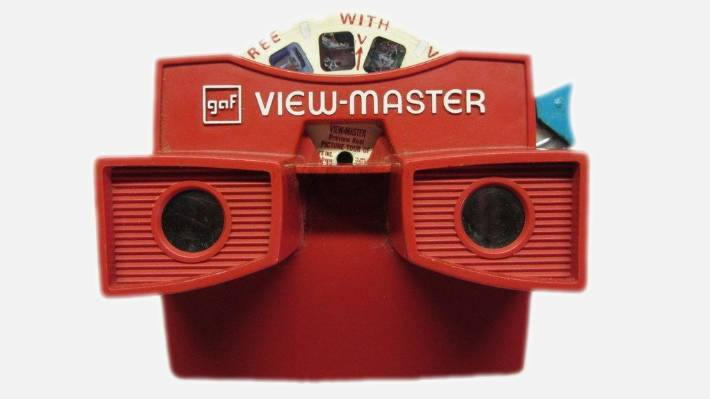
\includegraphics[width=\linewidth]{viewmaster.jpg}
    \caption{De View-Master, uitgebracht in 1939 \autocite{ViewMaster}}
    \label{fig:viewmaster}
\end{figure}

\begin{figure}
    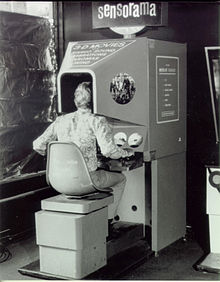
\includegraphics[width=\linewidth]{sensorama.jpg}
    \caption{De Sensorama van Morton Heilig, de machine speelde een video af en stimuleerde de zintuigen met geuren, wind, water... om zo teleprescence op te wekken \autocite{Chen2015}}
    \label{fig:sensorama}
\end{figure}

\section{Teleprescence}
Een grote fout die veel mensen maken is Virtual Reality koppelen aan hardware terwijl dit veel meer is \autocite{Steuer1992}. 
Tijdens het gebruik van een \acrshort{vr} applicatie is de gebruiker aanwezig in 2 "werelden", dit noemt men teleprescence.

Uit de definitie van \autocite{Steuer1992} kan men ook afleiden dat er twee manieren zijn om teleprescence op te wekken. De eerste is maken dat de gebruiker zich niet bewust is van de virtuele wereld en hier helemaal in ondergedompeld is, wat dus eigenlijk een vorm van escapisme is. De andere manier is om ervoor te zorgen dat de virtuele wereld geen aparte wereld is maar deel uitmaakt van de echte wereld. Als men met deze manier werkt moet de applicatie de virtuele elementen op zo'n natuurlijk mogelijke manier integreren in de echte wereld. 
% TODO CONTENT Perceptie van automatische en gecontrolleerde mentale processen

Teleprescence komt niet alleen voor bij VR maar bij elke applicatie die een communicatiemedium gebruikt. Dit medium is niet alleen digitaal maar ook fysieke zaken zoals kranten kunnen je het gevoel geven dat je er echt 'aanwezig' bent, mensen ervaren dit soms als rillingen wanneer ze bijvoorbeeld iets choquerend lezen. 
Een groot verschil tussen VR en de andere mediums waarbij teleprescence in meespeelt is dat bij VR de gebruiker beide zender en ontvanger is. Hij zal acties versturen naar de virtuele wereld en beelden terugkrijgen op basis van zijn acties.
Aan de hand van deze definitie kunnen we dus afleiden dat zelfs 360 graden video's ook als VR tellen. Dit is omdat de beelden die de gebruiker te zien krijgt afhangen van de draaihoek hoe hij kijkt naar het scherm, zelfs telefoneren kan men eigenlijk zien als VR \autocite{Steuer1992}.
Omdat deze definitie van VR heel ruim is, beperkt deze bachelorproef zich tot de technologieën die gebruik maken van een gyroscoop of andere sensoren om zo een betere ervaring te geven. Het begrip VR is met de opkomst van \acrfull{hmd} meer gelinkt aan het aanwezig zijn in een pure virtuele wereld. Voor deze reden is er een nieuwe term tot leven geroepen genaamd \acrfull{xr}. Deze term is een overkoepeling van alles dat te maken heeft met \acrlong{ar}, \acrlong{vr} en \acrlong{mr}.

Om het niveau van teleprescence bij de gebruiker te verhogen zijn volgende twee variabelen belangrijk: de immersie / echtheid en de interactiviteit van de applicatie \autocite{Steuer1992}.
De belangrijkste factor die de echtheid van een applicatie verhoogt is de stimulatie van de zintuigen. Wanneer de gebruiker bijvoorbeeld echt de wind en het water voelt terwijl hij in een virtuele regen staat zal hij misschien meer geneigd zijn om de virtuele wereld als echt te gaan ervaren \autocite{Steuer1992}. De invloed van deze externe factoren kan afhangen van gebruiker tot gebruiker, sommige gebruikers staan hier meer voor open en zullen zich sneller ondergedompeld voelen in de ervaring dan anderen.
Voor het verhogen van de interactiviteit zijn er verscheidene mogelijkheden, de gekozen manier zal vaak afhangen van de gekozen technologie. Een \acrshort{hmd} implementeert dit door de gebruiker beide handen te laten gebruiken om acties uit te voeren. Deze acties kunnen dan gebeuren door het herkennen van de lichaamsdelen of door externe controllers.

Het herkennen van een een lichaamsdeel komt voor wanneer de software effectief het lichaamsdeel zelf herkent en niet a.h.v. sensoren bevestigd op het lichaamsdeel. Om gebruik te maken van deze techniek is er wel een camera nodig die bevestigd is aan de voorkant van het apparaat (HoloLens, Smartphone) of een externe camera die lichaamsdelen herkent, bijvoorbeeld Microsoft Kinect \autocite{Ren2013}.
Meestal zal een applicatie de vorm van een hand proberen te detecteren, a.h.v. deze vorm kan dan een 'gesture' worden herkend die dan gelinkt is aan een bepaalde actie \autocite{Piumsomboon2013}. 
Voor het herkennen van gestures is er de mogelijkheid om computer vision te gebruiken \autocite{Ji2013}.


Alhoewel deze twee variabelen een grote rol spelen bij teleprescence is het doel van de applicatie ook zeer belangrijk. Een goed voorbeeld hiervan is Pokémon GO. Bij het bestuderen van de implementatie van de twee variabelen hierbij ziet men het volgende. De interactiviteit van de app is redelijk simpel, de spelers lopen rond in de echte wereld door hun gps te gebruiken en kunnen zo op het scherm een beweging doen om monsters te vangen. Realisme is dan geïmplementeerd door gebruik te maken van augmented reality, deze plaatst dan de monsters in de echte wereld. Deze twee implementaties zijn dus eigenlijk niet zo geavanceerd en kwamen al voor in andere apps (Ingress), maar toch is Pokémon GO veel succesvoller dan deze andere apps. Dit komt vooral omdat Pokémon GO voldoet aan de verwachte ervaring van de gebruiker, namelijk een echte trainer zijn zoals in de Pokémon games en serie \autocite{Tang2017}. Hieruit volgt dus de conclusie dat de graad waarop deze variabelen zijn geïmplementeerd zal afhangen van de use case. Ook speelde het sociale aspect een grote rol in het continue succes van Pokémon GO, dit kan dus ook als een mogelijke invloed gezien worden waar er rekening mee moet worden gehouden \autocite{Tang2017}.


Het is dus voor deze reden dat deze studie een derde variabele toevoegt, namelijk de bruikbaarheid voor de gekozen use case. Net zoals bij de 2 variabelen van \textcite{Steuer1992} bestaat deze uit 3 subcategorieën namelijk: praktisch, financieel en logisch. Aan de hand van de twee voorafgaande variabelen en deze nieuwe wordt er in de longlist bepaald welke technologie er verder besproken wordt a.h.v. een shortlist met verschillende frameworks. 

\section{Computer Vision}
Vooral bij Augmented of Mixed Reality zal men te maken krijgen met computer vision. Computer vision is interdisciplinair wetenschappelijk gebied dat verschillende domeinen bevat in verband met herkenning a.h.v. beeldmateriaal. Waaronder: 

\begin{itemize}
    \item Herkennen van afbeeldingen
    \item Herkennen van objecten
    \item Herkennen van bewegingen
    \item Aanpassen van foto- en beeldmateriaal om zo ruis te verwijderen
\end{itemize}

Vele van deze algoritmen maken gebruik van artificiële intelligentie, een vaak gebruikte techniek hiervoor is 'convolutional neural network' \autocite{Ji2013}. Afhankelijk van het algoritme zal dit neuraal netwerk opzoek gaan naar features (een herkenbaar punt) die nuttig zijn. Bij gezichtsherkenning is het vinden van de neus, ogen en randen van het gezicht (zie figuur \ref{fig:cnnface}) belangrijk terwijl een automatische drone eerder wilt weten waar de obstakels zich bevinden. Met de gevonden features kan de applicatie dan het gezicht blijven volgen en een filter hierop toepassen of kan er een 3D object worden gemaakt (bijvoorbeeld een obstakel) in het geval van de drone. 

Het gebruik van computer vision wordt later verder besproken in de secties \ref{sec:augmentedreality} en \ref{sec:mixedreality}.

\begin{figure}
    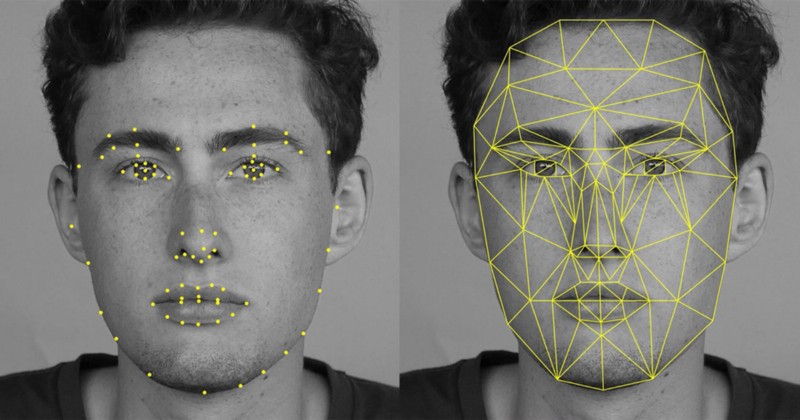
\includegraphics[width=\linewidth]{cnnFace.jpeg}
    \caption{Herkennen van features om zo een digitaal gezicht te maken \autocite{Murray2017}}
    \label{fig:cnnface}
\end{figure}

\section{Degrees Of Freedom}

XR technologieën kunnen ook nog eens worden onderverdeeld afhankelijk van het aantal vrijheidsgraden dat ze ondersteunen. In de wereld van XR komen \acrshort{3dof} en \acrshort{6dof} het meeste voor. Deze vrijheidsgraden bepalen in welke mate de gebruiker kan bewegen in de virtuele wereld \autocite{Chen1995}.

\acrshort{3dof} ondersteunt alleen rotationele bewegingen, deze zijn: yaw, pitch en rol. Deze hebben echter alleen maar de mogelijkheid om de camera te draaien en niet van locatie te veranderen. Bij \acrshort{6dof} is dit wel mogelijk omdat deze over volgende bewegingen beschikt: up and down, front and back en left and right (zie figuur \ref{fig:dof}).
Een technologie met \acrshort{6dof} heeft wel de mogelijkheid om in de virtuele wereld rond te lopen, alsook zal de mogelijkheid er nog altijd zijn om te camera te draaien omdat 6DOF beschikt over rotationale en positionele bewegingen. De ondersteuning van deze vrijheidsgraden ligt niet alleen bij de technologie zelf maar ook bij de gebruikte hardware \autocite{Chen1995}. In de longlist zal er in detail worden besproken hoeveel vrijheidsgraden ondersteund zijn en welke hardware er juist nodig is om ze te gebruiken.

\begin{figure}
    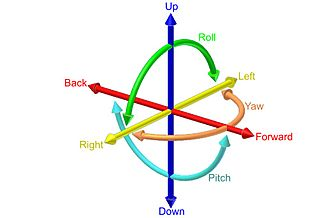
\includegraphics[width=\linewidth]{dof.jpg}
    \caption{\acrfull{6dof} \autocite{6dofImage}}
    \label{fig:dof}
\end{figure}

% TODO CONTENT Uitleg IMU

\section{Gelijkaardige use cases}
% TODO CONTENT Gelijkaardige use case
\subsection{Cleveland Museum of Art}\label{ch:cleveland}
Dit museum maakt gebruik van software genaamd ArtLens. Artlens bestaat uit verschillende onderdelen die gebundeld zijn in één dezelfde smartphone app. Met deze app kunnen bezoekers een interactieve tour krijgen. In het museum bevinden zich bluetooth beacons waardoor de app kan weten waar de bezoeker zich bevindt en zo tonen waar het volgende kunstwerk is. Ook kan de gebruiker zijn interesses opgeven waardoor de app voorstellen kan doen van kunstwerken die dichtbij zijn. 
De bezoekers kunnen ook zelf hun eigen tours maken en deze delen met andere gebruikers wat dan weer het sociale aspect van de applicatie bevordert.

Het VR gedeelte van deze applicatie bestaat uit de mogelijkheid om informatie over een schilderij te tonen wanneer de gebruiker met zijn camera op het schilderij mikt.
In het museum bevinden zich ook terminals waar de gebruikers hun smartphone op kunnen leggen. Hierdoor verschijnt er op een groot scherm een opdracht die de gebruiker dan moet uitvoeren: bijvoorbeeld het nadoen van een schilderij of na een tijdje het schilderij zo goed mogelijk proberen te schilderen \autocite{Ding2017}.

\subsection{Smithsonian}
Bij het Smithsonian wordt er ook gebruikgemaakt van augmented reality, deze keer door gebruik te maken van BroadcastAR. Deze software gebruikt een camera om zo te streamen naar een groot scherm waar de bezoekers dan de AR-objecten kunnen zien. Het nadeel van deze implementatie is dat er weinig of geen interactie is tussen de gebruiker en de software. 

Het Smithsonian heeft ook nog een tweede augemented reality app waarbij gebruikers hun camera kunnen richten op skeletten om zo het skelet om te toveren naar een 3D-model van het levend dier.

\subsection{Historium Brugge}
Het Historium in Brugge maakt geen gebruik van augemented reality maar wel van virtual reality. De applicatie biedt twee soorten ervaringen aan, City VR en Historium VR. Bij City VR kan de gebruiker verschillende locaties van Brugge bezoeken in VR, terwijl hij bij Historium VR een interactive rondeleiding krijgt over het middeleeuwse Brugge. De City VR applicatie kan worden geïnstalleerd op elke smartphone die AR ondersteund, voor Historium VR is er echter wel een VR headset inclusief controllers nodig. 

\subsection{\acrlong{muhka}}
Het \acrshort{muhka} heeft vroeger geëxperimenteerd met ErfgoedApp om zo met bluetooth beacons (tonen informatie wanneer de bezoeker dichtbij is) en augmented reality het niveau van hun museum op te krikken. De bezoekers van het \acrshort{mukha} waren echter niet zo geïnteresseerd in het downloaden van een applicatie eens ze in het museum aankwamen. 

Wat de ErfgoedApp wel heel goed doet is de manier waarop musea kunstwerken kunnen toevoegen \autocite{ErfgoedApp}. Door gebruik te maken van een website kunnen zij afbeeldingen uploaden en hieraan verschillende zaken linken zoals:

\begin{enumerate}
    \item Video
    \item Info
    \item Muziek
\end{enumerate}  

Deze app is wel beperkt in het creëren van een virtuele wereld. Het is alleen mogelijk om zaken te linken aan een afbeelding en niet om virtuele objecten te creëren.